

We now introduce GP related theory and notations.
We work exclusively with two-variable regression problems.
Let the data be pairs of real-valued scalars $\{(x_i,y_i)\}_{i=1}^n$ (complete data will be denoted by column vectors $\mathbf{x}$, $\mathbf{y}$).
In regression, one tries to learn a functional relationship $y_i = f(x_i)$, where the function $f$ is to be learned.
GPs present a non-parametric way to express prior knowledge on the space of possible functions $f$.
Formally, a GP is an infinite-dimensional extension of the multivariate Gaussian distribution.
For any finite set of inputs $\xbf$, the marginal prior on $f(\xbf)$ is the multivariate Gaussian
\[
f(\xbf) \sim \mathcal{N}(m(\xbf), k(\xbf,\xbf)),
\]
where $m(\xbf) = \Ebkt[f]{f(\xbf)}$ is the mean function and $k(\xbf,\xbf') = \Cov_f\pn{f(\xbf), f(\xbf')}$ is the covariance function, a.k.a.\ kernel.\footnote{
  Note that $m(\xbf) = \pn{m(x_i)}_{i=1}^{n}$ and $k(\xbf,\xbf') = \begin{pmatrix} k(x_i,x'_{i'}) \end{pmatrix}^{1 \leq i \leq n}_{1 \leq i' \leq n'}$, where $n'$ is the number of entries in $\xbf'$.
}
Together $m$ and $k$ characterize the distribution of $f$; we write
\[ f \sim \mathcal{GP}(m,k). \]
In all examples below, our prior mean function $m$ is identically zero; this is the most common choice.
The marginal likelihood can be expressed as:
\begin{equation}
\label{eq:marg}
p\pn{f(\xbf) = \ybf \mvert \xbf} = \int p\pn{f(\xbf) = \ybf \mvert f, \xbf}\, p(f|\xbf) \, df
\end{equation}
where here $p(f|\xbf) = p(f) \sim \mathcal{GP}(m,k)$ since we assume no dependence of $f$ on $\xbf$.
We can sample a vector of unseen data $\ybf^* = f(\xbf^*)$ from the predictive posterior with
\begin{equation}
\label{eq:gpsampler}
\ybf^* \sim \mathcal{N}(\bm{\mu},\bm{\Sigma}),
\end{equation}
a multivariate normal with mean vector
\begin{equation}
\label{eq:conditonalGaussianMean}
\bm{\mu} = k(\xbf^*,\xbf)\, k(\xbf,\xbf)^{-1}\, \ybf
\end{equation}
and covariance matrix
\begin{equation}
\label{eq:conditonalGaussianCovariance}
\bm{\Sigma} =  k(\xbf^*,\xbf^*) - k(\xbf^*,\xbf)k(\xbf,\xbf)^{-1} k(\xbf,\xbf^*).
\end{equation}

Often one assumes the values $\ybf$ are noisily measured, that is, one only sees the values of $\ybf_\noisy = \ybf + \wbf$ where $\wbf$ is Gaussian white noise with variance $\sigma_\noise^2$.
In that case, the log-likelihood is
\begin{equation}
\log p\pn{\ybf_\noisy \mvert \xbf} =
-\frac12 \ybf^\top (\bm{\Sigma}
+ \sigma_\noise^2 \Ibf)^{-1} \ybf
- \frac12\log \abs{\bm{\Sigma} + \sigma_\noise^2 \Ibf}
- \frac{n}{2}\log 2\pi
\end{equation}
where $n$ is the number of data points.
Both log-likelihood and predictive posterior can be computed efficiently in a Venture SP with an algorithm that resorts to Cholesky factorization\citep[chap. 2]{rasmussen2006gaussian} resulting in a computational complexity of $\mathcal{O}(n^3)$ in the number of data points.



The covariance function governs high-level properties of the observed data such as linearity, periodicity and smoothness.
The most widely used form of covariance function is the squared exponential:
\begin{equation}
  k(x,x^\prime) = \sigma^2 \exp\pn{-\frac{(x-x^\prime)^2}{2\ell^2}},
\end{equation}
where $\sigma$ and $\ell$ are hyperparameters: $\sigma$ is a scaling factor and $\ell$ is the typical length-scale.

Adjusting hyperparameters results in a new covariance function with the same qualitative human-interpretation; more drastically different covariance functions are achieved by changing the structure of the covariance function.
%A different type could be a linear covariance function:
%\begin{equation}
% k(x,x^\prime) = \sigma^2 (x-\ell) (x^\prime-\ell). 
%\end{equation}
Note that covariance function structures are compositional: adding or multiplying two valid covariance functions results in another valid covariance function. 

It has been suggested that adding covariance structures $k_1,k_2$ together,
\begin{equation}
k_3(x,x^\prime) = k_1(x,x^\prime) + k_2(x,x^\prime),
\end{equation}
corresponds to combining global structures, while multiplying covariance functions,
\begin{equation}
k_4(x,x^\prime) = k_1(x,x^\prime) \times k_2(x,x^\prime),
\end{equation}
corresponds to combining local structures~\citep{duvenaud2013structure}.
Note that both $k_3$ and $k_4$ are valid covariance function structures.






Venture includes the primitive \texttt{make\_gp}, which takes as arguments a
unary function \texttt{mean} and a binary (symmetric, positive-semidefinite)
function \texttt{cov} and produces a function $\gtt$ distributed as a Gaussian
process with the supplied mean and covariance.  For example, a function $\gtt
\sim \GP(0,\,\SE)$, where $\SE$ is a squared-exponential covariance
\[ \SE(x, x') = \sigma^2 \exp\pn{\frac{(x-x')^2}{2\ell}} \]
with $\sigma=1$ and $\ell=1$, can be instantiated as follows:
\begin{lstlisting}[language=Venture]
assume zero = make_const_func( 0.0)
assume se = make_squaredexp( 1.0, 1.0)
assume g  = make_gp( zero, se)
\end{lstlisting}
There are two ways two view $\gtt$ as a ``random function.'' In the first view,
the \texttt{assume} directive that instantiates $\gtt$ does not use any
randomness---only the subsequent calls to $\gtt$ do---and coherence constraints
are upheld by the interpreter by keeping track of which evaluations of $\gtt$
exist in the current trace.  Namely, if the current trace contains evaluations
of $\gtt$ at the points $x_1,\ldots,x_N$ with return values $y_1,\ldots,y_N$,
then the next evaluation of $\gtt$ (say, jointly at the points $x_{N+1}, \ldots,
x_{N+n}$) will be distributed according to the joint conditional distribution
\[
  P\pn{\big.
    \texttt(\gtt\ x_{N+1}\texttt), \ldots, \texttt(\gtt\ x_{N+n}\texttt)
    \mvert
    \texttt(\gtt\ x_i\texttt) = y_i \text{ for $i=1,\ldots,N$}}.
\]
In the second view, $\gtt$ is a randomly chosen deterministic function, chosen
from the space of all deterministic real-valued functions; in this view, the
\texttt{assume} directive contains \emph{all} the randomness, and subsequent
invocations of $\gtt$ are deterministic.  The first view is procedural and is
faithful to the computation that occurs behind the scenes in Venture.  The
second view is declarative and is faithful to notations like ``$g \sim P(g)$''
which are often used in mathematical treatments.  Because a model program could
make arbitrarily many calls to $\gtt$, and the joint distribution on the return
values of the calls could have arbitrarily high entropy, it is not
computationally possible in finite time to choose the entire function $\gtt$ all
at once as in the second view.  Thus, it stands to reason that any
computationally implementable notion of ``nonparametric random functions'' must
involve incremental random choices in one way or another, and Gaussian processes
in Venture are no exception.

Behind the scenes, Venture attaches a state $D = (\xbf_\past, \ybf_\past)$ to
each procedure created by \texttt{make\_gp}, where $\xbf_\past$ is a vector of
all past inputs to $\gtt$ in the current trace, and $\ybf_\past$ is the
corresponding vector of outputs.  (The state $D$ is updated each time an
invocation of $\gtt$ is added to or removed from the current trace.)  Thus, the
incremental random choices made by a GP $\gtt$ in Venture are simply samples
from the conditional distribution $P\pn{\gtt \mvert D}$.  That is, if $\gtt$ was
initialized as \texttt{make\_gp mean cov)} and has accrued state $D =
(\xbf_\past, \ybf_\past)$, then
\[
\texttt{(g }\xbf\texttt{)}
\sim
P\pn{
  \texttt{(g}_0\ \xbf\texttt{)}
  \mvert
  \texttt{(g}_0\ \xbf_\past\texttt{)} = \ybf_\past
}, \qquad\text{where $\gtt_0 \sim \texttt{make\_gp mean cov)}$}.
\]

Statefully represented random functions highlight the difference between
\texttt{predict} and \texttt{sample} (see Section \ref{sec:interactivity}).  To
illustrate, consider the following program:

\begin{mdframed}
\begin{lstlisting}[language=Venture,escapechar=\#]
assume zero = make_const_func( 0.0)
assume se =  make_squaredexp( 1.0, 1.0)
assume g = make_gp( zero, se)

call_back( draw_gp_curves( g( ...)))
#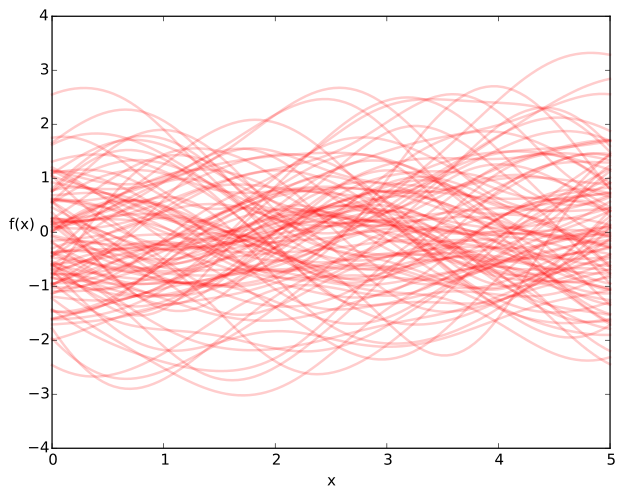
\includegraphics[width=10cm]{figs/interactive_gp_prior.png}#
sample( g( array(1 2 3)))
\\ [-1.04331626 -0.72016875 -0.44525212]
call_back( draw_gp_curves( g( ...)))
#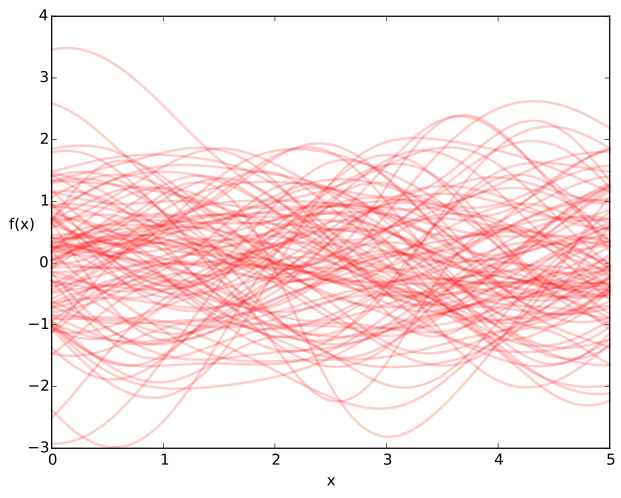
\includegraphics[width=10cm]{figs/interactive_gp_after_sample.png}#
predict( g( array(1 2 3)))
\\ [ 0.55736593  0.09784888  0.56553757]
call_back( draw_gp_curves( g( ...)))
#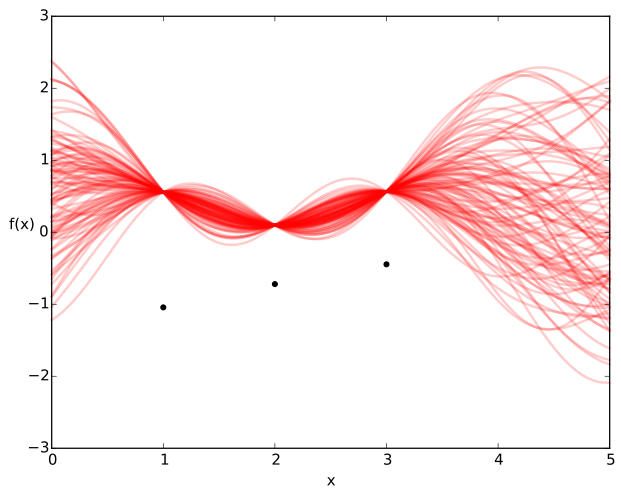
\includegraphics[width=10cm]{figs/interactive_gp_after_predict.png}#
\end{lstlisting}
\end{mdframed}
(The callback \texttt{draw\_gp\_curves} draws a cloud of curves sampled from
$\gtt$.)  The \texttt{sample} directive does not affect the state of $\gtt$, so
the distribution of $\gtt$ after the \texttt{sample} is the same as the prior.
The \texttt{predict}, however, does affect the state; the distribution of $\gtt$
after the \texttt{predict} directive is conditioned on the values returned by
$\gtt$ inside the directive.  This explains why, in the final plot, all curves
go through the points returned by the previous \texttt{predict} directive, and
do not go through the points returned by the \texttt{sample} directive (which
are marked with black dots for reference).


